\chapter{Implementación del protocolo LoRaLAN}\label{chap:5}

En este capítulo se indaga en los detalles propios de la implementación del protocolo. Se describe el entorno de programación, el hardware sobre el que se programa, las librerías en las que se apoya el desarrollo, los elementos de los que se compone la librería, la interfaz de programación y otros detalles que merecen ser nombrados.

\section{Entorno de desarrollo y plataforma hardware}\label{sec:entorno}

El hardware sobre el que se diseña y se desarrolla el protocolo es el microcontrolador ESP32 de Espressif. Se decide que este actúe como nodo de la red. Se eligió por ser el microcontrolador actual por excelencia en IoT y porque reúne en un solo procesador dos núcleos de procesamiento. Además, ofrece una memoria suficiente para mantener toda la lógica del protocolo y de aplicaciones propias y una implementación de mecanismos criptográficos AES y CMAC a través de mbedTLS, lo que evita tener que incorporar una biblioteca de cifrado externa. La disponibilidad de dos núcleos se aprovecha en el prototipo de registro de asistencia, donde la radio se atiende en una tarea fijada al núcleo~0 mientras que la lectura de tarjetas, los sensores y la pantalla se ejecutan en el bucle principal del núcleo~1, de forma que ninguna operación lenta de los periféricos retrasa la respuesta del nodo a la pasarela.

Como transceptor se ha utilizado el SX1276, en su versión breakout (adaptada para trabajar en protoboards) de Semtech, un circuito de la familia SX127x que implementa la modulación LoRa y que se comunica con el microcontrolador mediante un bus SPI, al que se añade una línea de reinicio y la línea de interrupción DIO0, por la que el chip señaliza el fin de una transmisión o de una recepción. A todos los equipos se les asigna una misma configuración de red con los mismos parámetros de radio, recogidos en el fichero \texttt{config.h} de cada programa, que son una frecuencia de 869,525~MHz, un ancho de banda de 125~kHz, un factor de ensanchamiento SF7, una tasa de codificación 4/5, una palabra de sincronización \texttt{0x12}, una potencia de 14~dBm y un preámbulo de 8~símbolos.

El gateway de la red se ejecuta sobre una Raspberry Pi 4 a la que se conectó, de nuevo, un segundo módulo SX1276 por el bus SPI0 del conector de 40~pines, de manera que el mismo equipo aloja el proceso de la pasarela LoRaLAN, el servidor de la aplicación y la base de datos, sin necesidad de un ordenador adicional en la instalación. Para las pruebas se emplearon además otras dos placas, una LilyGo T3 V1.6, que integra un ESP32 y un SX1276 en la misma placa y que se programó como nodo simulado para disponer de un segundo nodo sin montar otro prototipo completo, y un M5Stack Cardputer con el módulo Cap LoRa-1262, que incorpora un transceptor SX1262 de la familia más reciente de Semtech y que se programó como monitor pasivo, capaz de escuchar y descifrar el tráfico de la red sin transmitir en ningún momento.

Un SX1262 y SX1276 son transceptores completamente distintos y, aun así, los dos pueden funcionar con el mismo código gracias a la capa de abstracción que proporciona RadioLib.

La librería \textbf{RadioLib} es una biblioteca de código abierto escrita en C++ que ofrece controladores para un gran número de transceptores, entre ellos los de las familias SX127x y SX126x. Todos sus controladores derivan de una clase base común, \texttt{PhysicalLayer}, que expone las operaciones genéricas de una radio, como transmitir, iniciar la recepción o explorar el canal, y el acceso al hardware se realiza a través de una capa de adaptación a la plataforma, denominada HAL, de la que la propia biblioteca incluye implementaciones para Arduino y para la Raspberry Pi. De esta forma, se pudo codificar el protocolo una sola vez y ejecutarlo tanto en un microcontrolador como en un ordenador con Linux, sin reescribir el acceso a la radio en cada caso. 

El firmware de los nodos se desarrolló con el IDE de Arduino, al que se añadió el soporte de placas de Espressif. Se optó por este entorno, y no ESP-IDF, porque el \textit{framework} de Arduino simplifica la configuración de los dispositivos y porque la mayoría de las bibliotecas de los sensores y del lector NFC del prototipo están publicadas para este entorno.

El gateway, en cambio, no se compila con el IDE de Arduino, sino como un programa nativo de Linux construido con CMake y con el compilador g++ de la propia Raspberry Pi. El proyecto incorpora las fuentes de RadioLib y de LoRaLAN, utiliza el HAL \texttt{PiHal} de RadioLib, que accede a los pines mediante la biblioteca lgpio y al bus SPI mediante el controlador \texttt{spidev} del \textit{kernel}, y se enlaza con mbedTLS para disponer del cifrado AES-128 real. Ya que la biblioteca LoRaLAN incluye la cabecera \texttt{Arduino.h}, que no existe en Linux, el proyecto aporta una versión propia de esa cabecera en el directorio \texttt{src/compat}, que implementa sobre primitivas POSIX las pocas funciones que el protocolo necesita, como \texttt{millis()} a partir del reloj del sistema, de forma que la biblioteca se compila sin ninguna modificación.

El mismo principio se aplicó para disponer de un simulador de PC que pudiera evaluar el rendimiento del protocolo. La idea de utilizar un simulador para testear LoRaLAN surge de lo tedioso que resulta cargar las distintas versiones del firmware sobre los prototipos y de la simpleza del montaje que se dispone para evaluar elementos que afectan al protocolo como es el canal radioeléctrico o el número de nodos que transmiten. El simulador se compila en Windows con el g++ de MSYS2, que ejecuta la pasarela y varios nodos en un único proceso sobre un canal virtual con pérdidas y colisiones y que sustituye \texttt{Arduino.h}, \texttt{RadioLib.h} y mbedTLS por versiones simuladas. Esta herramienta permite repetir un mismo escenario de forma determinista con un canal radioeléctrico virtual antes de llevarlo al hardware.

De esta manera se ha podido disponer de una biblioteca que funciona en tres entornos distintos, el ESP32, la Raspberry Pi y un PC, sin que su código contenga grandes dependencias, más allá de las ligeras adaptaciones en las dependencias utilizadas. 

Para que el protocolo pueda utilizarse desde cualquier boceto con una simple directiva \texttt{\#include}, se empaquetó siguiendo la especificación de bibliotecas del IDE de Arduino, que requiere un directorio con el nombre de la biblioteca que contenga el código fuente en un subdirectorio \texttt{src} y un fichero de metadatos \texttt{library.properties}, con el nombre, la versión, el autor, las arquitecturas compatibles y las dependencias. Opcionalmente puede incluir un directorio \texttt{examples} con bocetos de ejemplo. En LoRaLAN se declara \texttt{architectures=*}, ya que el código no depende de ningún microcontrolador concreto, y \texttt{depends=RadioLib}, de modo que el gestor del IDE ofrece instalar esta dependencia junto con la biblioteca. La biblioteca se instala copiando el directorio en la carpeta \texttt{libraries} del usuario o mediante la opción «Añadir biblioteca .ZIP».

Por último, el código se gestionó con Git en un único repositorio que contiene la biblioteca, el simulador, el prototipo y esta memoria. Durante el desarrollo se contó con la asistencia de herramientas de inteligencia artificial generativa como apoyo a las tareas de programación en C++. Su utilización se limitó a facilitar la implementación y resolución de problemas de desarrollo, manteniéndose bajo responsabilidad del autor las decisiones de diseño, la integración del código y la verificación de su funcionamiento.

\section{Arquitectura de la librería}

Como ya se ha comentado, la librería que permite emplear el protocolo LoRaLAN está escrita en C++. A la hora de codificar el protocolo se tuvo en mente que la librería debe ser fácil de utilizar, con un código mantenible y modular. Como resultado, se han obtenido seis módulos presentados a continuación con las responsabilidades que abarcan, en la Tabla~\ref{tab:modulos}.

\begin{table}[H]
\centering
\caption{\label{tab:modulos} Módulos de la librería LoRaLAN.}
\begin{tabular}{|p{3.4cm}|p{10.4cm}|}
\hline
\textbf{Módulo} & \textbf{Responsabilidad} \\
\hline
\texttt{LoRaLANCrypto} & Primitivas criptográficas sobre mbedTLS: cifrado AES-128-CTR, CMAC truncado, derivación de la clave de sesión, construcción del bloque inicial del contador. \\
\hline
\texttt{LoRaLANPacket} & Formato de trama (construcción, análisis y validación estructural), gestión del MIC y constructores de tramas de gestión. \\
\hline
\texttt{LoRaLANManager} & Cifrado y descifrado de la carga útil, numeración de secuencia y lógica de transmisión fiable (espera de ACK, plazos, retransmisiones). \\
\hline
\texttt{LoRaLANDevice} & Recepción y autenticación de tramas, selección de la clave del MIC, emisión de confirmaciones, escucha del canal y gestión de la ventana de secuencia. \\
\hline
\texttt{LoRaLANGateway} & Lógica de gateway (tabla de nodos, asociación, gestión de sondeo por turno, difusión de la hora, órdenes y confirmación diferida). \\
\hline
\texttt{LoRaLANNode} & Lógica de nodo (asociación, eventos con escucha previa y retroceso, respuesta al sondeo, recepción de órdenes y rescate de eventos). \\
\hline
\end{tabular}
\end{table}

La primera versión de la librería reunía toda la lógica en un único fichero, con más de 20 bifurcaciones según el rol, nodo o gateway, de modo que cada cambio en uno obligaba a revisar el otro. Por este motivo, se reestructuró en una clase base, \texttt{LoRaLANDevice}, que contiene lo que ambos papeles hacen igual, y en dos clases derivadas, \texttt{LoRaLANGateway} y \texttt{LoRaLANNode}, que aportan únicamente lo propio de cada uno. Para comprobar que el cambio no alteró el comportamiento del protocolo.
La Figura~\ref{fig:uml-loralan} muestra el diagrama de módulos UML resultante.

\begin{figure}[H]
\centering
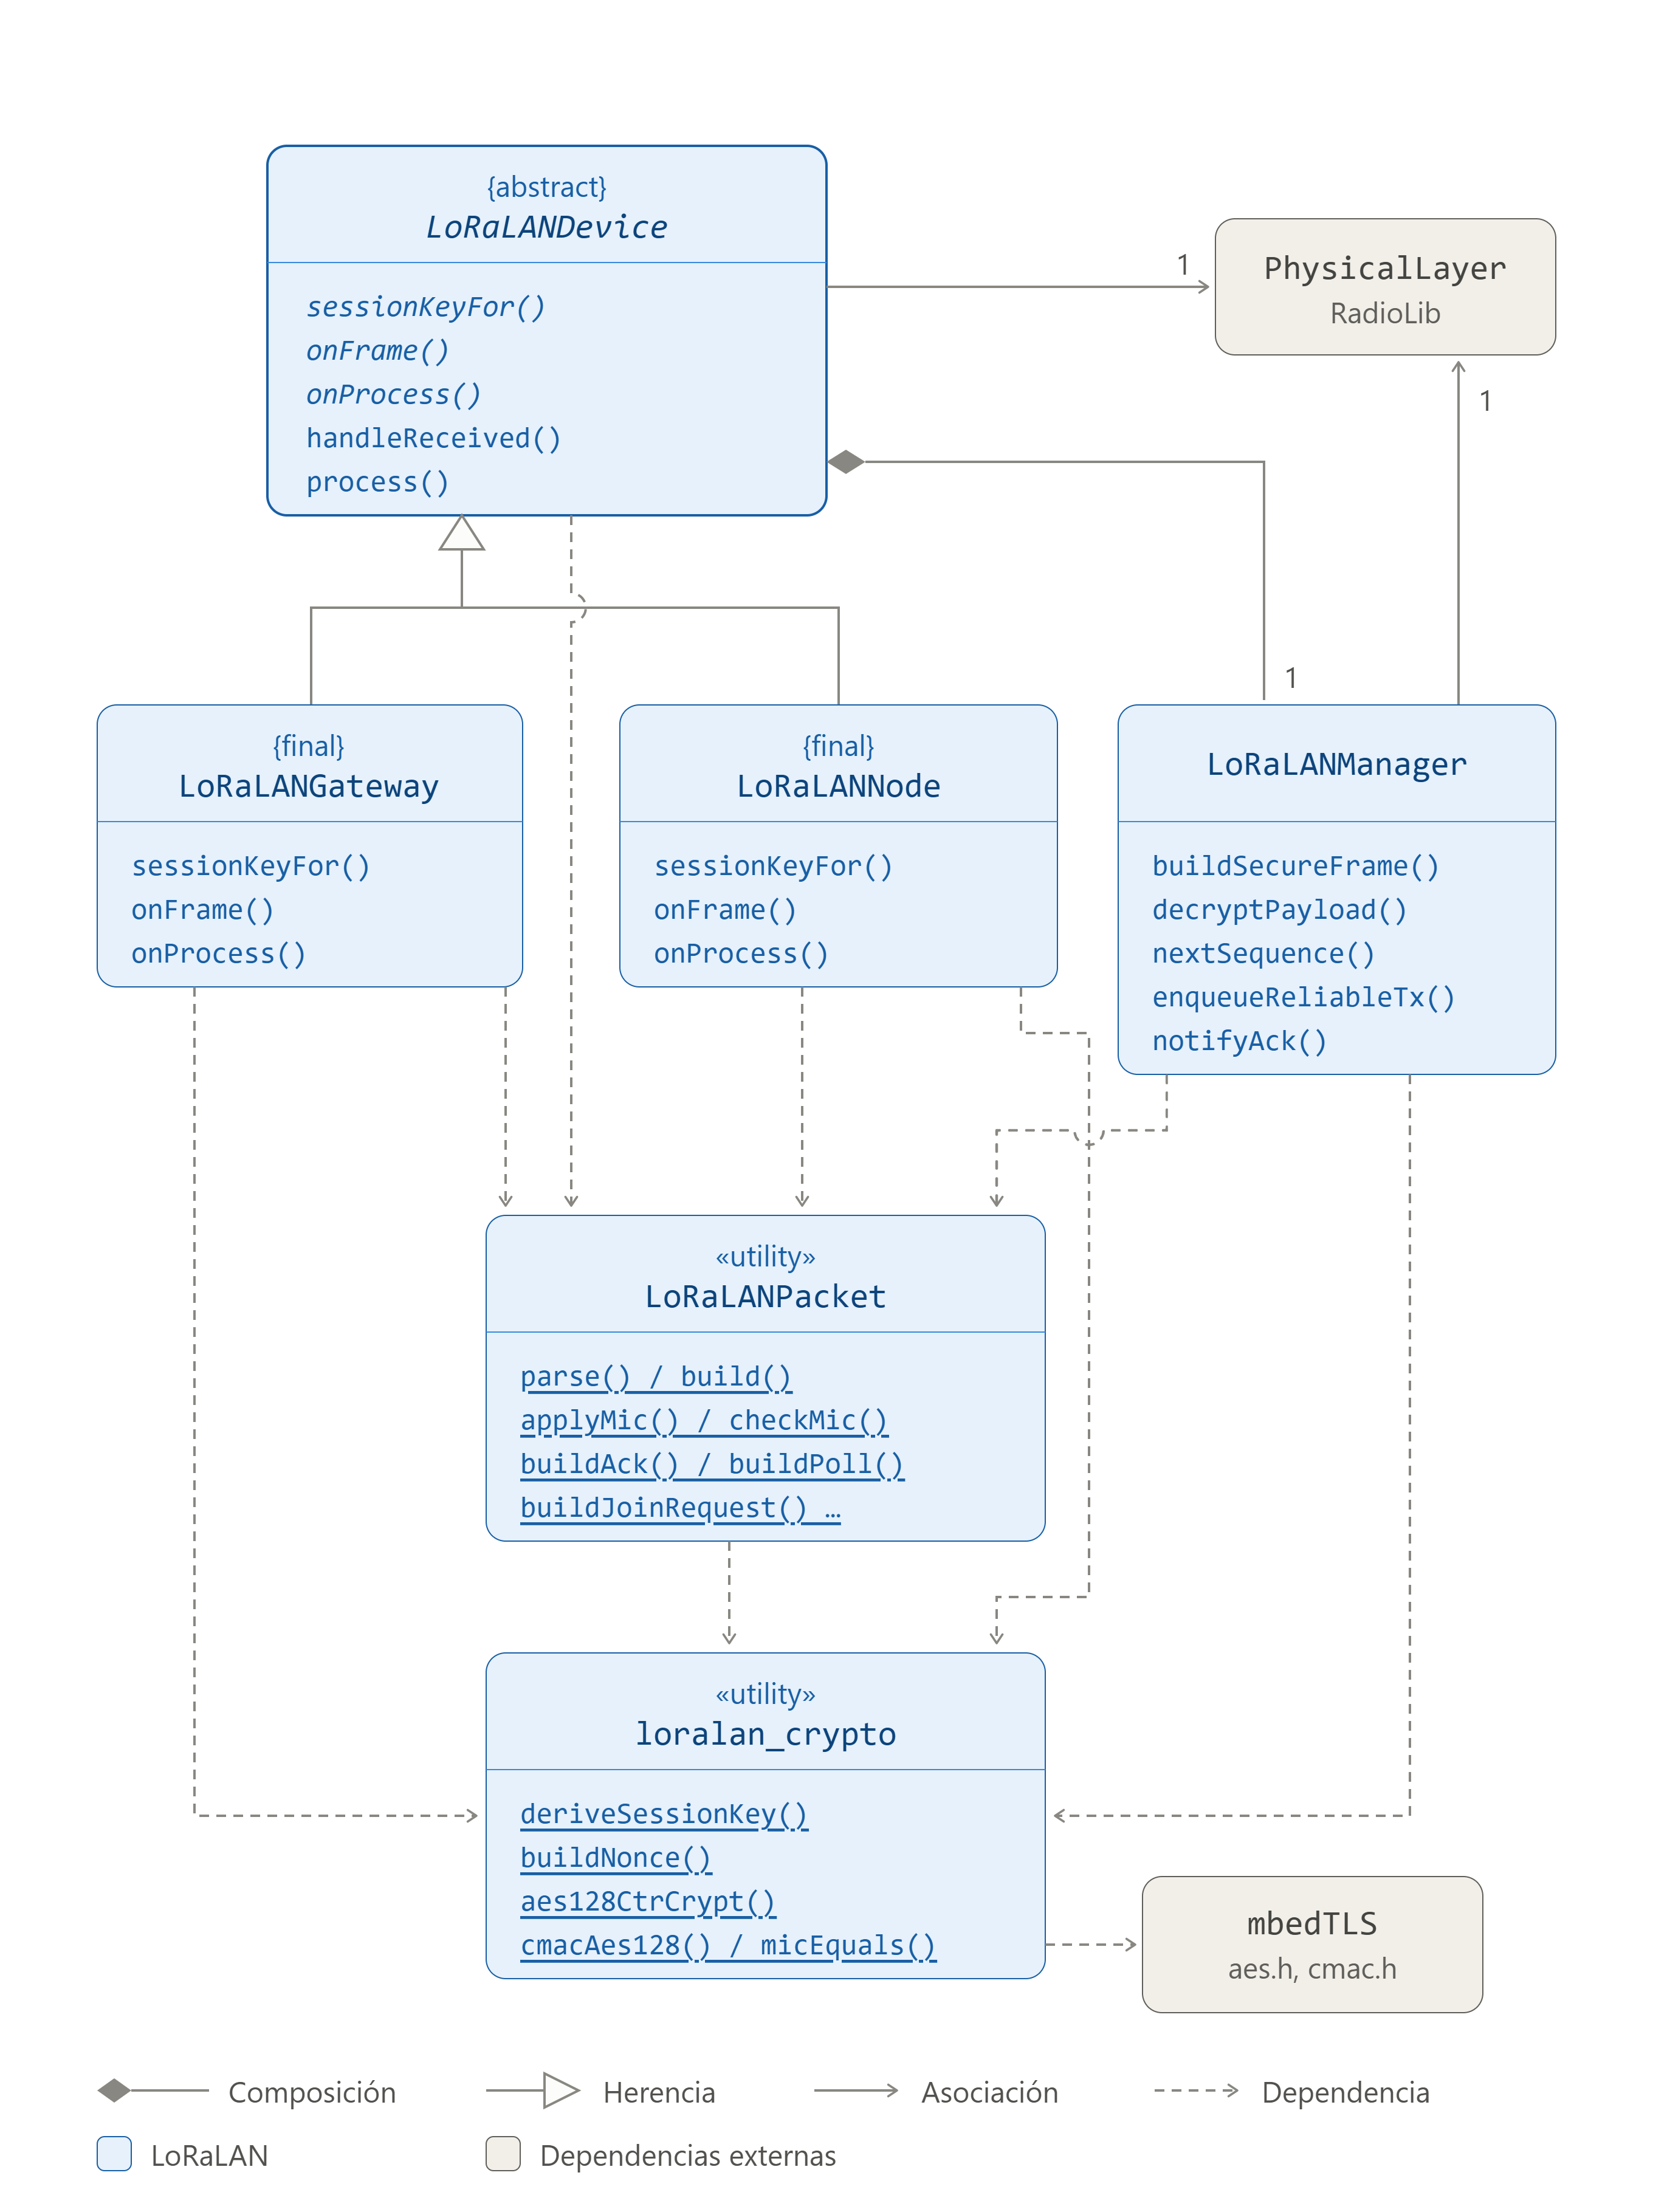
\includegraphics[width=0.95\textwidth]{imagenes/loralan_diagrama_clases_v6.png}
\caption{\label{fig:uml-loralan} Diagrama de módulos UML de la librería LoRaLAN.}
\end{figure}

La lógica de recepción de paquetes se concentra en el módulo base, que comprueba la estructura del paquete, el identificador de red y verifica el MIC antes de entregarlo al rol correspondiente, de forma que una trama sin autenticar no llega a descifrarse ni modifica el estado del dispositivo. En la transmisión, los paquetes que no esperan confirmación se envían directamente, mientras que los que sí la esperan quedan a cargo de \texttt{LoRaLANManager}, que gestiona los plazos y las retransmisiones y que admite un único envío fiable en curso, decisión que simplifica el código a costa de limitar el rendimiento de cada dispositivo.

La librería accede a la radio únicamente a través de \texttt{PhysicalLayer}, la clase base de RadioLib. Por último, su código no reserva memoria dinámica por sí mismo, con la salvedad de la que pueda emplear internamente mbedTLS, ya que todas las estructuras tienen un tamaño fijo y residen dentro de los propios objetos, de manera que la tabla de nodos que emplea el gateway, con 32 entradas de 108~bytes en la compilación para PC, ocupa unos 3,4~kB y en ella se realizan búsquedas lineales, debido a su reducido tamaño.

\section{Interfaz de programación}\label{sec:api}

La interfaz se ha diseñado de modo que la puesta en marcha de un dispositivo sea lo más sencilla posible. Para ello, se crea, en primer lugar, un objeto sobre una radio de RadioLib, se rellena una estructura de configuración, se registran las funciones de retrollamada\footnote{Las funciones de retrollamada o \textit{callbacks} son aquellas que la aplicación define y registra en la librería para que sea esta quien las ejecute cuando se produce un determinado suceso, como la llegada de un paquete.} que interesen y, en el bucle principal, se entregan al objeto los paquetes recibidos y se le llama periódicamente. Por ejemplo, en el Listado~\ref{lst:nodo} se muestra un nodo completo, que se asocia por sí solo y que, a partir de ese momento, envía eventos y responde a los sondeos.


\begin{lstlisting}[language=C++,basicstyle=\ttfamily\footnotesize,frame=single,breaklines=true,breakatwhitespace=true,caption={Ejemplo de implementación de un nodo LoRaLAN.},label={lst:nodo},captionpos=b]
// Transceptor LoRa.
SX1276 radio = new Module(PIN_CS, PIN_DIO0, PIN_RST, RADIOLIB_NC);
LoRaLANNode node(radio);     // nodo LoRaLAN sobre esa radio

// Llamada al recibir una orden valida del gateway
void onCommand(const LoRaLANFrame& frame,
               const uint8_t* payload, uint8_t payloadLen) {
  // orden del gateway, ya descifrada
}
// Llamada al cerrarse un evento push (entregado o no)
void onPushAck(bool delivered,
               const uint8_t* ackPayload, uint8_t ackLen) {
  // desenlace del evento y respuesta de la aplicacion
}

void setup() {
  // 869.525 MHz, BW 125 kHz, SF7, CR 4/5, sync 0x12,
  // 14 dBm, preambulo de 8 simbolos
  int st = radio.begin(869.525, 125.0, 7, 5, 0x12, 14, 8);
  if (st != RADIOLIB_ERR_NONE)
    while (true) {}          // radio no disponible

  // Parametros de red y credenciales del nodo
  LoRaLANNode::Config cfg;
  cfg.netId  = 0x42;         // identificador de la red
  cfg.nodeId = 0x10;         // preferida; 0 = cualquiera
  memcpy(cfg.hwId, MAC, LORALAN_HWID_SIZE);  // id fisico
  cfg.appKey = APP_KEY;      // clave de 16 bytes
  node.begin(cfg);

  // Registro de callbacks de la aplicacion
  node.setOnCommand(onCommand);
  node.setOnPushAck(onPushAck);
  radio.startReceive();      // radio en escucha continua
}

void loop() {
  // 1) Recepcion: se entrega cada trama a la libreria
  if (radio.checkIrq(RADIOLIB_IRQ_RX_DONE) == 1) {
    uint8_t buffer[LORALAN_HEADER_SIZE + LORALAN_MAX_PAYLOAD
                   + LORALAN_MIC_SIZE];  // trama maxima
    size_t len = radio.getPacketLength();
    if (len <= sizeof(buffer) &&
        radio.readData(buffer, len) == RADIOLIB_ERR_NONE)
      node.handleReceived(buffer, len);
    radio.startReceive();    // volver a escuchar
  }

  // 2) Temporizadores, reintentos y envios pendientes
  node.process();

  // 3) Encolado de eventos de la aplicacion
  if (hasEvent && node.queuePushEvent(data, dataLen))
    hasEvent = false;        // la libreria ya tiene su copia
}
\end{lstlisting}


El gateway sigue el mismo patrón, como se observa en el Código~\ref{lst:gateway}, que muestra únicamente la configuración y las operaciones propias del gateway, omitiéndose la inicialización de la radio y la recepción de tramas, que se realizan igual que en el Código~\ref{lst:nodo}. En él se activa la confirmación diferida para que la aplicación responda a cada evento cuando dispone del resultado, que viaja dentro del propio ACK.

\begin{lstlisting}[language=C++,basicstyle=\ttfamily\footnotesize,frame=single,caption={Ejemplo de uso de la librería desde un gateway con confirmación diferida.},label={lst:gateway},captionpos=b]
LoRaLANGateway gateway(radio);

void onPushEvent(const LoRaLANFrame& frame,
                 const uint8_t* payload, uint8_t payloadLen) {
  // se anota (frame.header.srcId, frame.header.seq) y se consulta al servidor
}

void setup() {
  // radio.begin(...) y startReceive() igual que en el nodo
  LoRaLANGateway::Config cfg;
  cfg.netId           = 0x42;
  cfg.gatewayId       = 0x00;
  cfg.appKey          = APP_KEY;
  cfg.pollIntervalMs  = 5000;        // cumple la sub-banda del 10 %
  cfg.deferredPushAck = true;
  gateway.begin(cfg);
  gateway.setOnPushEvent(onPushEvent);
}

void loop() {
  // recepcion igual que en el nodo, con gateway.handleReceived(...)
  gateway.process();                 // POLL, TIME_SYNC y reintentos de CMD
}

// Cuando llega el resultado del servidor para (nodeId, seq):
void onResultado(uint8_t nodeId, uint16_t seq, uint8_t code) {
  gateway.ackPush(nodeId, seq, &code, 1);   // code 0 = OK; otro = NACK
}

// Orden a un nodo; false si ya hay otra 
// en curso o el nodo no esta asociado:
bool enviarOrden(uint8_t nodeId, const uint8_t* cmd, uint8_t len) {
  return gateway.sendCommand(nodeId, cmd, len);
}
\end{lstlisting}


Las operaciones comunes a los dos roles son las siguientes:

\begin{itemize}
\item \textbf{\texttt{begin(config)}}: Aplica la estructura de configuración y reinicia el estado de asociación, lo que en el gateway supone vaciar la tabla de nodos, sin transmitir nada, ya que el nodo inicia la asociación desde \texttt{process}.

\item \textbf{\texttt{handleReceived(buffer, len)}}: Entrega al protocolo un paquete de \texttt{len} bytes recibido por la radio y devuelve \texttt{false} si es inválido, si pertenece a otra red, si no se dispone de clave para su origen, si no supera la verificación del MIC o si se rechaza.

\item \textbf{\texttt{process()}}: Atiende los plazos, las retransmisiones y las tareas periódicas, por lo que debe llamarse continuamente desde el bucle principal.
\end{itemize}

Por su parte, las operaciones principales del nodo son las que se enumeran a continuación:

\begin{itemize}
\item \textbf{\texttt{queuePushEvent(payload, payloadLen, ackRequired, fallbackToPoll)}}: Encola un evento, que se transmite desde \texttt{process} tras escuchar el canal. El parámetro \texttt{ackRequired}, activo por defecto, solicita confirmación, mientras que \texttt{fallbackToPoll}, inactivo por defecto, rescata la carga para el siguiente sondeo si se agotan los intentos, sustituyendo a la que estuviera encolada para ese sondeo. Devuelve \texttt{false} si el nodo no está asociado, si la carga supera los 64~bytes o si ya hay un evento encolado.
\item \textbf{\texttt{queuePollPayload(payload, payloadLen, ackRequired)}}: Prepara la carga de la siguiente respuesta a un sondeo, sustituyendo a la que estuviera encolada. Con \texttt{ackRequired}, activo por defecto, la carga se conserva hasta recibir el ACK. Devuelve \texttt{false} si el nodo no está asociado o si la carga supera los 64~bytes.

\item \textbf{\texttt{requestJoin()}}: Reactiva la asociación automática, que se realiza desde \texttt{process}.

\item \textbf{\texttt{leave()}}: Solicita la baja mediante una trama con confirmación, desactiva la asociación automática y borra la clave de sesión al recibir el ACK o al agotarse los intentos. 
\item \textbf{\texttt{isJoined()}}: Indica si el nodo está asociado.
\item \textbf{\texttt{setOnCommand(cb)}}: Registra la función que recibe las órdenes del gateway ya descifradas.
\item \textbf{\texttt{setOnPushAck(cb)}}: Registra la función que recibe el desenlace de cada evento con confirmación, con los parámetros \texttt{delivered}, que indica si llegó el ACK, y \texttt{ackPayload} y \texttt{ackLen}, que contienen la respuesta de la aplicación. No se invoca si la sesión se pierde antes de conocerse el desenlace.
\item \textbf{\texttt{setOnPollRequest(cb)}}: Registra la función que genera la respuesta a un sondeo cuando no hay ninguna carga encolada.
\item \textbf{\texttt{setOnJoinAccepted(cb)}}: Registra la función a la que se avisa cuando se acepta la asociación.
\end{itemize}

En cuanto al gateway, sus operaciones principales son las siguientes:

\begin{itemize}
\item \textbf{\texttt{sendCommand(nodeId, payload, payloadLen)}}: Envía a \texttt{nodeId} una orden cifrada, con confirmación y reintentos. Devuelve \texttt{false} si el nodo no está asociado, si la carga supera los 64~bytes o si hay otro envío fiable en curso.

\item \textbf{\texttt{ackPush(nodeId, seq, payload, payloadLen)}}: Envía la confirmación del evento \texttt{seq} del nodo \texttt{nodeId}, con una respuesta de aplicación opcional. Devuelve \texttt{false} si ese evento ya no está pendiente.

\item \textbf{\texttt{nodeCount()}}: Devuelve el número de nodos asociados y activos.

\item \textbf{\texttt{isAlive(nodeId, maxAgeMs)}}: Indica si el nodo está asociado y si se ha recibido de él un evento, una respuesta a un sondeo o una solicitud de asociación en los últimos \texttt{maxAgeMs} milisegundos.

\item \textbf{\texttt{nodeHwId(nodeId, out)}}: Copia en \texttt{out} el identificador de fábrica del nodo y devuelve \texttt{false} si este no figura en la tabla.

\item \textbf{\texttt{setOnPushEvent(cb)}, \texttt{setOnPollResponse(cb)}}: Registran las funciones que reciben, ya descifrados, los eventos y las respuestas a los sondeos de los nodos, teniendo en cuenta que estas últimas pueden llegar vacías.

\item \textbf{\texttt{setOnNodeJoined(cb)}, \texttt{setOnNodeLeft(cb)}, \texttt{setOnNodeInactive(cb)}}: Registran las funciones a las que se avisa, con la dirección del nodo, cuando este se asocia, se da de baja o deja de contestar a los sondeos.
\end{itemize}

Los parámetros de temporización son configurables y disponen de los valores por defecto que se recogen en la Tabla~\ref{tab:temporizacion}.

\begin{table}[H]
\centering
\caption{\label{tab:temporizacion} Parámetros de configurables y valores por defecto.}
\begin{tabular}{|l|l|p{6.6cm}|}
\hline
\textbf{Parámetro} & \textbf{Valor} & \textbf{Significado} \\
\hline
\texttt{appAckTimeoutMs} & 1200~ms & Espera de la confirmación tras cada transmisión. \\
\hline
\texttt{appMaxRetries} & 3 & Transmisiones máximas totales: la inicial y dos retransmisiones. \\
\hline
\texttt{joinRetryMs} & 5000~ms & Intervalo entre solicitudes de asociación, sin máximo de intentos. \\
\hline
\texttt{timeSyncIntervalMs} & 30000~ms & Intervalo entre difusiones de la hora. \\
\hline
\texttt{pollIntervalMs} & 2000~ms & Intervalo entre sondeos. \\
\hline
\texttt{maxMissedPolls} & 3 & Sondeos sin respuesta para declarar inactivo un nodo. \\
\hline
\texttt{silenceTimeoutMs} & 0 & Detección de silencio del nodo, desactivada por defecto. \\
\hline
\end{tabular}
\end{table}

Los sondeos cada 2000~ms suponen por sí solos, en SF7, un 2,06~\% de ciclo de trabajo, sin contar el resto de las tramas del gateway. La detección de silencio se deja desactivada porque su plazo depende del número de nodos y del periodo de sondeo de cada instalación.

Debe tenerse en cuenta que un valor de retorno \texttt{true} en las operaciones de envío significa únicamente que la petición se ha aceptado, y no que la trama haya llegado a su destino. Asimismo, las cargas que se entregan a estas operaciones se copian o se transmiten durante la propia llamada, por lo que la aplicación no necesita conservarlas después.

Los \textit{callbacks} se ejecutan de forma síncrona dentro de la llamada a \texttt{handleReceived} o a \texttt{process} que los origina, y los punteros que reciben solo son válidos mientras dura la función, de modo que su contenido debe copiarse si se necesita más adelante o desde otro hilo. Puesto que una operación lenta en ellos retrasa la recepción, los plazos, las retransmisiones y las tareas periódicas, el gateway del prototipo no realiza en sus \textit{callbacks} ninguna operación de red y se limita a encolar los datos para que los atiendan otros hilos, tal como se describe más adelante.

En cuanto a las confirmaciones, se distinguen dos tipos:

\begin{itemize}
\item \textbf{Confirmación automática}: Se envía al retornar el \textit{callback}, para toda trama aceptada que la solicite y vaya dirigida al dispositivo, mientras que el emisor espera 1200~ms por defecto, más un retardo aleatorio de hasta 600~ms, antes de retransmitir.

\item \textbf{Confirmación diferida}: Se aplica a los eventos con confirmación cuando \texttt{deferredPushAck} está activo, de modo que el ACK no se envía al retornar el \textit{callback}, sino cuando la aplicación llama a \texttt{ackPush}. Mientras no lo haga, las retransmisiones del nodo quedan sin respuesta, por lo que la aplicación debe contestar antes de que este agote sus intentos y, a ser posible, antes de su primera retransmisión, lo que en el prototipo se garantiza con la cadena de plazos del apartado~\ref{sec:gwlinux}.
\end{itemize}

Por último, la librería no inicializa la radio ni detecta la llegada de los paquetes, sino que es la aplicación la que configura el transceptor, decide si atiende la recepción por interrupción o por consulta y entrega cada trama al protocolo, aunque la transmisión y la exploración del canal sí se realizan desde la librería. Gracias a ello, esta se integra tanto en el bucle de un programa de Arduino como en la tarea de FreeRTOS del nodo o en el hilo de radio del gateway, si bien no incorpora mecanismos de exclusión mutua, por lo que todas las llamadas a un mismo objeto deben realizarse desde un único hilo. Debe considerarse, además, que la transmisión y la exploración del canal son bloqueantes, de modo que las llamadas que las realizan se prolongan al menos durante el tiempo en el aire de la trama, lo que ha de tenerse en cuenta si ese hilo asume otras tareas.

\section{Implementación del nodo en la aplicación registro de asistencia}\label{sec:nodo-app}

En este apartado se describe cómo se ha implementado el firmware del nodo en el sistema de fichaje que se desarrolla en el trabajo. El nodo conserva el hardware del sistema de partida, formado por un ESP32, un lector NFC PN532, los sensores BME280, BH1750 y LD2410, una pantalla OLED, dos relés, tres LED y un zumbador, y añade un transceptor SX1276 que comparte el bus SPI con el lector. Puesto que el nodo debe atender a la vez el protocolo de radio y todos estos periféricos, el mayor riesgo es que una operación lenta, como una lectura por I$^2$C o el refresco de la pantalla, interfiera en la comunicación. Por eso, se aprovechan los dos núcleos del ESP32, de manera que todo lo relativo a la radio se concentra en una tarea fijada al núcleo~0, mientras que la gestión de la aplicación se ejecuta en el núcleo~1, como se muestra en la Figura~\ref{fig:nodo-tareas}.

\begin{figure}[H]
\centering
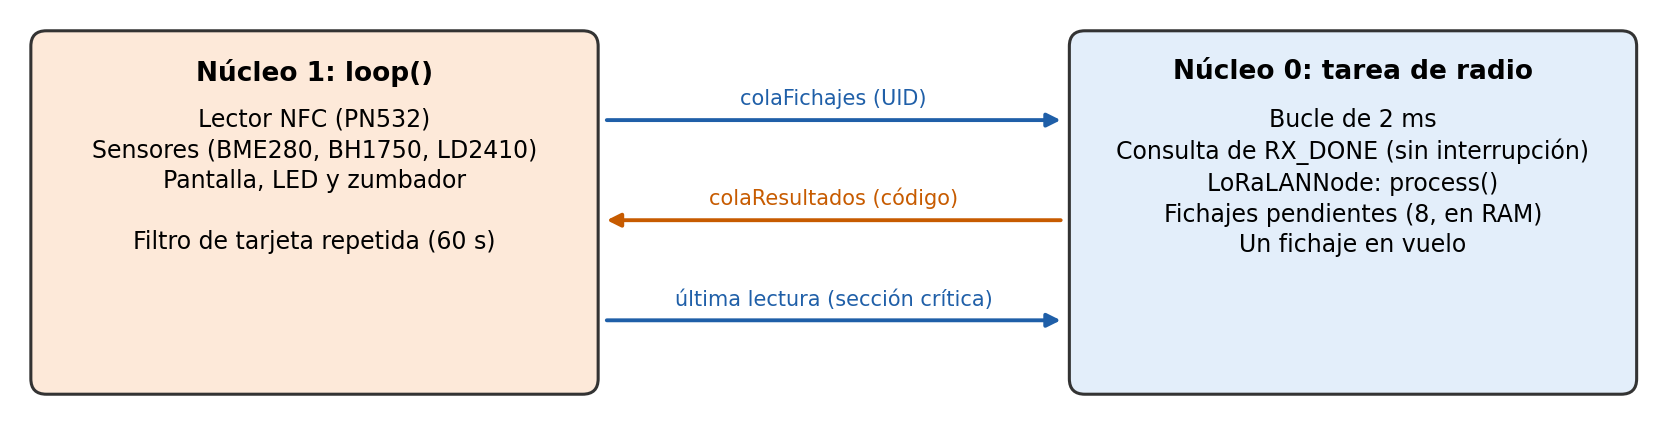
\includegraphics[width=0.88\textwidth]{imagenes/nodo_tareas.png}
\caption{\label{fig:nodo-tareas} Reparto del firmware del nodo entre los dos núcleos del ESP32.}
\end{figure}

Ambos núcleos se comunican sin bloquearse mediante dos colas del sistema operativo, una para los fichajes leídos y otra para sus resultados, y una copia de la última lectura de los sensores protegida frente al acceso simultáneo. La tarea de radio repite cada 2~ms el mismo ciclo, en el que comprueba si ha llegado una trama, la entrega a \texttt{handleReceived} y llama a \texttt{process}. Para detectar paquetes se consulta el registro de estado del transceptor en lugar de emplear su interrupción, debido a que la detección de actividad de canal señala el fin de la exploración (\textit{CadDone}) por la misma línea DIO0 y provocaría falsas recepciones.

Sobre esta estructura, cada función de la aplicación utiliza el mecanismo de la biblioteca que mejor se adapta a ella. Un fichaje se envía mediante \texttt{queuePushEvent} y su resultado llega en la respuesta de aplicación del ACK, que se obtiene a través de \texttt{setOnPushAck} y que distingue si el fichaje se ha registrado, si se ha rechazado de forma definitiva o si debe reintentarse. Las lecturas de los sensores y el estado de los relés se generan bajo demanda en la función registrada con \texttt{setOnPollRequest} y no solicitan confirmación, puesto que una lectura perdida se sustituye por la del sondeo siguiente. Por último, las órdenes del gateway llegan a través de \texttt{setOnCommand} y actúan sobre los relés o programan un reinicio, que se retrasa un segundo para que antes pueda enviarse el ACK de la propia orden.

Dado que la biblioteca admite un único evento encolado, la cola de fichajes pendientes es responsabilidad de la aplicación, que conserva hasta ocho fichajes en memoria RAM y mantiene uno solo en curso, de modo que el ACK recibido corresponde siempre al primero de la cola. Si no llega, el fichaje pasa al final de la cola y no vuelve a enviarse hasta pasados 30~s. Además, como la biblioteca descarta sin notificarlo el evento en curso cuando el nodo pierde la asociación, la aplicación deja de esperar su desenlace si detecta esa pérdida
o si transcurren 20~s sin conocerlo, y el primero de la cola se envía de nuevo en cuanto el nodo vuelve a estar asociado.

Al arrancar por primera vez, el nodo solicita una dirección dinámica y guarda en memoria no volátil la que le asigna el gateway. En los arranques siguientes solicita esa misma dirección y conserva su identidad en el servidor y, con ella, su aula. Por último, se activa la detección de silencio con un plazo equivalente a tres vueltas de sondeo, el máximo admitido, y el intervalo de sondeo de 5~s del gateway, de modo que, si el gateway se reinicia y deja de reconocer al nodo, este repite la asociación hasta que el gateway responde.

\section{Gateway sobre Linux en Raspberry Pi}\label{sec:gwlinux}

Implementar el gateway sobre un microcontrolador presenta una limitación práctica a la hora de comunicarse con el servidor, debido a que la pila de red y la radio compiten por el mismo procesador. Por este motivo, para el sistema de registro de asistencia, el gateway se ha implementado como un proceso de Linux sobre una Raspberry Pi, con un módulo SX1276 conectado por SPI.

La adaptación sigue el procedimiento descrito anteriormente. Por un lado, una capa implementa las funciones del entorno Arduino sobre las del sistema operativo, empleando un reloj monótono que no salta cuando el sistema ajusta su hora. Por otro lado, se utiliza la adaptación para Raspberry Pi que RadioLib incluye para acceder al SPI y a las líneas de entrada y salida, de modo que la librería LoRaLAN se compila sin modificar.

El proceso reparte su trabajo en los tres hilos que se muestran en la Figura~\ref{fig:gw-hilos}, unidos mediante colas, con el fin de que la radio no espere nunca a una operación de red. Una petición HTTP lenta dentro del \textit{callback} de recepción retrasaría el ACK más allá del plazo del nodo, y de hecho este defecto existía en el primer puente desarrollado para ESP32, que realizaba la petición dentro del \textit{callback} con un plazo de tres segundos, frente a los 1,2~segundos que espera el nodo. A continuación se detallan las responsabilidades de cada hilo.

\begin{figure}[H]
\centering
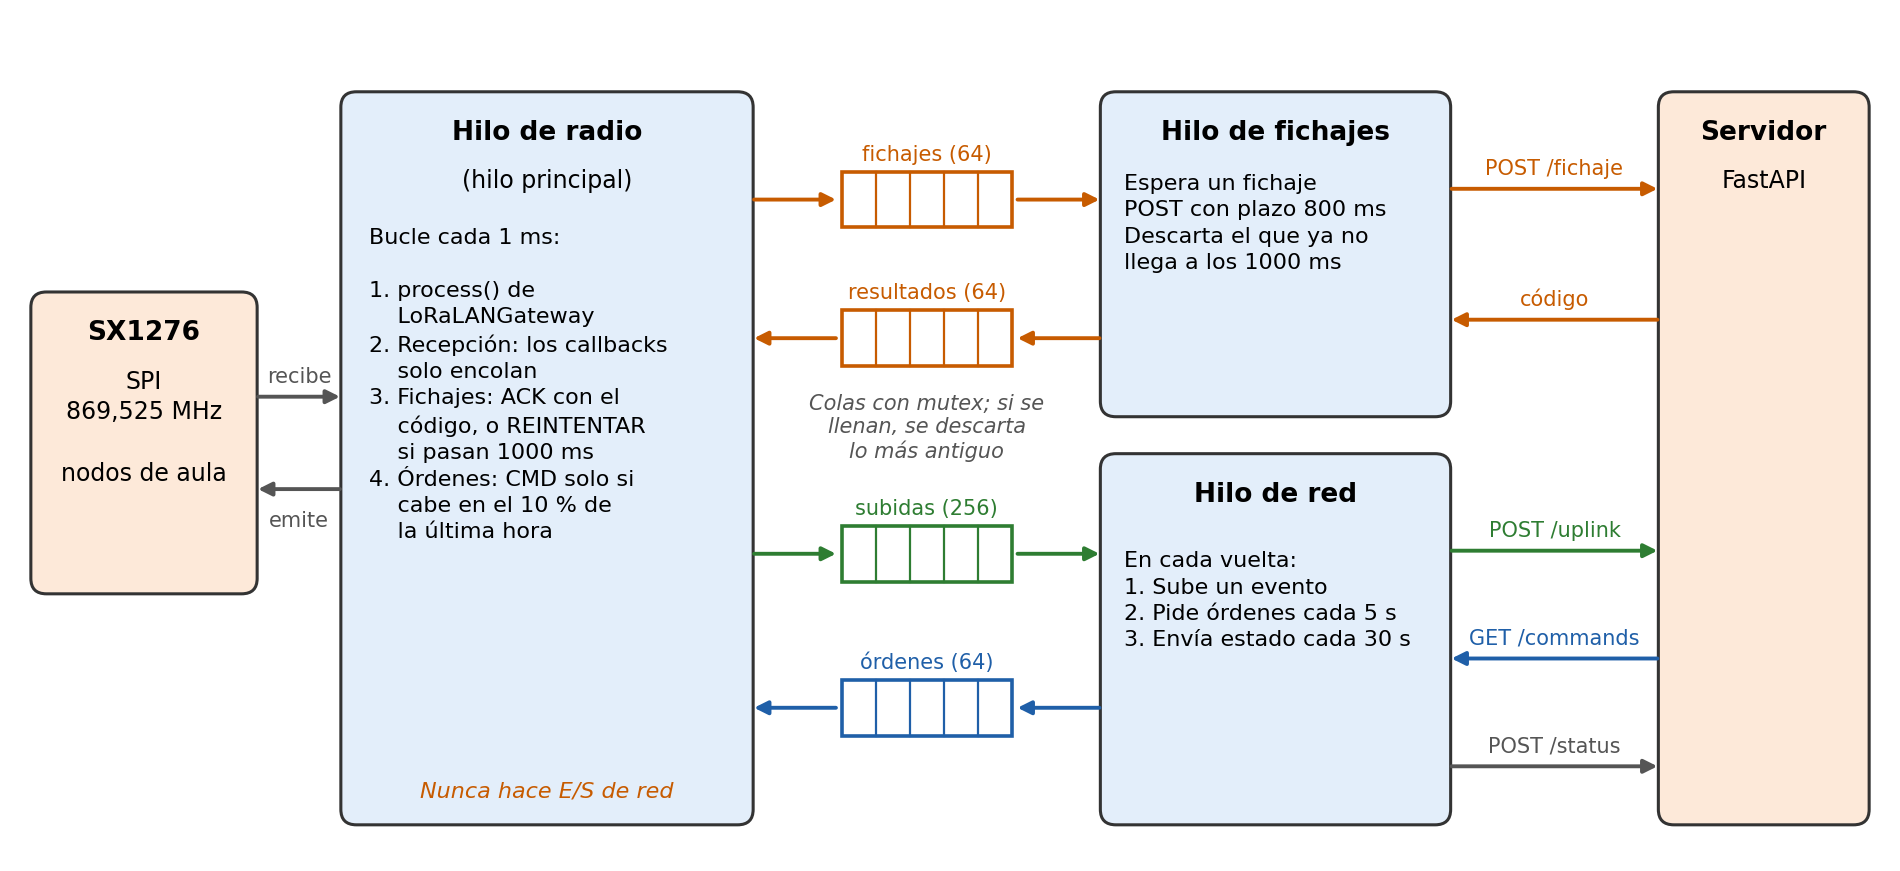
\includegraphics[width=0.88\textwidth]{imagenes/gateway_hilos.png}
\caption{\label{fig:gw-hilos} Hilos del gateway y colas que los unen.}
\end{figure}


\begin{itemize}
\item \textbf{Hilo de radio}: Ejecuta el protocolo y nunca realiza operaciones de red, ya que los \textit{callbacks} de la librería se limitan a encolar.

\item \textbf{Hilo de fichajes}: Consulta al servidor cada fichaje con un plazo de 800~ms y se separa del resto de comunicaciones para que una subida lenta de telemetría no le haga perder ese plazo.

\item \textbf{Hilo de red}: Sube la telemetría y las altas y bajas de nodos, recoge las órdenes del servidor cada 5~segundos y envía un informe de estado cada 30~segundos.
\end{itemize}

Si una cola se llena, se descarta el elemento más antiguo y se contabiliza en el informe de estado, puesto que perder una lectura antigua es preferible a detener la radio. La traducción entre el formato binario de la radio y el JSON del servidor reside en un módulo sin entrada ni salida, probado en PC, que convierte en REINTENTAR cualquier respuesta del servidor que no sea un código reconocible.

El gateway incorpora, además, dos piezas para el control del ciclo de trabajo de las que la librería carece:

\begin{itemize}
\item \textbf{Cálculo del tiempo en el aire}: Obtiene el de cualquier trama a partir de su longitud y de los parámetros de radio, según la ecuación del fabricante (ec.~\ref{eq:toa}).

\item \textbf{Contador de ciclo de trabajo}: Registra en una ventana deslizante el tiempo en el aire de las transmisiones de la última hora e indica si una nueva cabe en el presupuesto.
\end{itemize}

Con ellas, el gateway realiza dos comprobaciones. En primer lugar, al arrancar calcula qué fracción del ciclo de trabajo consumirá el sondeo, que es el mayor consumidor de tiempo en el aire, y, si excede el límite de la sub-banda, \textbf{termina con un error} en lugar de emitir de más en silencio. En segundo lugar, durante la ejecución comprueba que cada orden cabe en el presupuesto antes de transmitirla y, en caso contrario, la retiene hasta que quepa. Como el ciclo de trabajo de la sub-banda es, como máximo, del 10\,\%, no se espera que se dé esta circunstancia salvo en despliegues con mucho tráfico de eventos.

\section{Skill para desarrollo de aplicaciones para LoRaLAN mediante IA generativa}\label{sec:skill}

La revolución de la inteligencia artificial generativa y el desarrollo agéntico han cambiado por completo la forma en la que se desarrolla software~\cite{willison2026agentic}. Por ello, se ha considerado conveniente que la biblioteca incluya una \textit{skill} destinada a apoyar el desarrollo de aplicaciones que empleen LoRaLAN.

Una \textit{skill} es un paquete autocontenido de instrucciones, scripts y
recursos, organizado en un directorio cuyo elemento central es un fichero
\texttt{SKILL.md}, que un agente de IA descubre y carga dinámicamente para
especializarse en una tarea concreta. Su carga es progresiva: el agente solo
conoce inicialmente el nombre y la descripción de cada \textit{skill}, lee las
instrucciones completas cuando la considera relevante y accede a los ficheros
adicionales únicamente si la tarea lo requiere, lo que permite ampliar sus
capacidades sin saturar la ventana de contexto \cite{anthropic2025skills}.

La \textit{skill} se distribuye con la biblioteca en el fichero skills/loralan/SKILL.md, que el IDE de Arduino ignora durante la compilación. Para utilizarla, basta con copiarla al directorio de \textit{skills} de la herramienta de desarrollo agéntico que se desee.

Su contenido reúne las características principales del protocolo, los patrones de uso de la biblioteca, sus restricciones y las instrucciones para ejecutar las pruebas con el simulador. De este modo, proporciona a los agentes de programación el contexto necesario para utilizar LoRaLAN correctamente, evitando que propongan métodos inexistentes o soluciones incompatibles con su diseño.

Esta guía no sustituye a la documentación de la biblioteca ni garantiza la corrección del código generado, que sigue requiriendo revisión y pruebas. Asimismo, debe mantenerse actualizada cuando cambie la interfaz de programación.


\section{Síntesis del capítulo}

En este capítulo se ha abordado la implementación de LoRaLAN como una biblioteca modular escrita en C++, separando la lógica del protocolo de los detalles específicos de cada plataforma. Para ello, se ha definido una arquitectura organizada en seis módulos y una API que facilita su integración en aplicaciones. Asimismo, se ha adaptado la biblioteca para su compilación y ejecución en distintos entornos, desde microcontroladores ESP32 hasta sistemas Linux y un simulador para ordenador.

A partir de esta implementación se han desarrollado un firmware de referencia para los nodos ESP32 y una aplicación de pasarela para Raspberry Pi. Esta última incorpora una arquitectura concurrente que desacopla las comunicaciones LoRa de las operaciones de red y mecanismos de control del ciclo de trabajo. Finalmente, se ha creado una \textit{skill} que proporciona a los agentes de programación información contextual sobre el protocolo y facilita su utilización durante el desarrollo de aplicaciones.